\documentclass[final]{beamer}
\usepackage[size=custom, width=122, height=91, scale=1.2]{beamerposter}
\usetheme{gemini}
\usecolortheme{msu}
\usepackage{tikz}
\usetikzlibrary{shapes.geometric, arrows.meta, positioning}

% Define styles for flowchart
\tikzstyle{flowbox} = [rounded rectangle, minimum width=4cm, minimum height=1.5 cm, text centered, draw=black, fill=blue!10, font=\small]
\tikzstyle{flowarrow} = [thick, ->, >=Stealth]

\usepackage{graphicx}
\usepackage{lmodern}
\usepackage{multicol}
\usepackage{enumitem}
\usepackage{ragged2e}

\title{Speech Emotion Recognition: Clustering and Deep Learning Approach to Detect Conflicting Emotions through Vocal Expressions}
\author{Imtela Islam, Nuhash Kabir Neeha, Nuzhat Rahman \\ Supervisor: Dibyo Fabian Dofadar}
\logoright{\includegraphics[height=8cm]{logos/bracu_logo_white.png}}
\footercontent{\hfill
  \href{mailto:imtela.islam@g.bracu.ac.bd}{imtela.islam@g.bracu.ac.bd}, \hspace{0.5cm}     
  \href{mailto:nuhash.kabir.neeha@g.bracu.ac.bd}{nuhash.kabir.neeha@g.bracu.ac.bd}, \hspace{0.5cm}        
  \href{mailto:nuzhat.rahman@g.bracu.ac.bd}{nuzhat.rahman@g.bracu.ac.bd }}

\begin{document}
\begin{frame}[t]

% --- Left Column ---
\begin{minipage}[t]{0.28\textwidth}
\begin{block}{Abstract}
As the dependence on automated systems increases, it is essential for machines to comprehend human emotions in order to enhance user experience and minimize failures in sectors such as virtual assistants, customer service, and emergency hotlines. Speech Emotion Recognition (SER) is crucial in this context, as it seeks to decode emotions expressed through vocal expressions. Nevertheless, current SER models face challenges in recognizing conflicting emotions when individuals express multiple feelings simultaneously. This research introduces a clustering and deep learning methodology that effectively identifies both primary and overlapping emotions, thereby making a more natural and emotionally intelligent human-computer interaction.

\end{block}

    
\begin{block}{Dataset Description and Preprocessing}
% Add dataset/preprocessing summary here
\begin{itemize}
    \item \textbf{CREMA-D:} Crowd-sourced Emotional Multimodal Actors Dataset
    \begin{itemize}
        \item 7,442 clips, 91 actors (48 male, 43 female)
        \item 6 emotions: Angry, Disgust, Fear, Happy, Neutral, Sad
    \end{itemize}
    \item \textbf{RAVDESS:} Ryerson Audio-Visual Database of Emotional Speech and Song
    \begin{itemize}
        \item 24 actors
        \item 7 emotions: calm, happy, sad, angry, fearful, disgust, and surprised
        \item Includes both speech and song
    \end{itemize}
    \item \textbf{SAVEE:} Surrey Audio-Visual Expressed Emotion
    \begin{itemize}
        \item 4 male British speakers
        \item 7 emotions: Angry, Disgust, Fear, Happiness, Sadness, Surprise, Neutral
        \item Detailed labeling of utterances
        \item Synchronized video/audio
    \end{itemize}
    \item \textbf{TESS:} Toronto Emotional Speech Set
    \begin{itemize}
        \item 2 female actors
        \item 200 target words
        \item 7 emotions: Angry, Disgust, Fear, Happiness, Pleasant Surprise, Sadness, Neutral
    \end{itemize}
\end{itemize}


\begin{itemize}
    \item \textbf{Preprocessing:} Audio files were resampled, padded/truncated, and features such as MFCCs, Mel-spectrogram, and Chroma were extracted and standardized to fixed dimensions for model input.
\end{itemize}
\end{block}

\begin{block}{Methodology}
\begin{figure}
    \centering
    \begin{tikzpicture}[node distance=2.5cm]

    % Nodes
    \node (input) [flowbox] {Input Audio};
    \node (features) [flowbox, below of=input] {Feature Extraction \\ (MFCCs, Mel-spectrogram, Chroma)};
    \node (ensemble) [flowbox, below of=features] {Deep Learning Ensemble \\ CNN + GRU + BiLSTM};
    \node (dense) [flowbox, below of=ensemble] {Dense Layer \\ (Primary Emotion)};
    \node (fuzzy) [flowbox, below of=dense] {Fuzzy c-means Clustering \\ (Conflicting Emotions)};
    \node (output) [flowbox, below of=fuzzy] {Output: \\ Primary + Conflicting Emotions + Conflict Score};
    
    % Arrows
    \draw [flowarrow] (input) -- (features);
    \draw [flowarrow] (features) -- (ensemble);
    \draw [flowarrow] (ensemble) -- (dense);
    \draw [flowarrow] (dense) -- (fuzzy);
    \draw [flowarrow] (fuzzy) -- (output);
    
    \end{tikzpicture}
    \caption{Flowchart of Methodology}
    \label{fig:methodology}
\end{figure}
\begin{center}

\end{center}

\end{block}

\end{minipage}
\hfill
% --- Center Column ---
\begin{minipage}[t]{0.42\textwidth}
\begin{block}{Initial Model and Results}
\vspace{5}
\begin{figure}
    \centering
    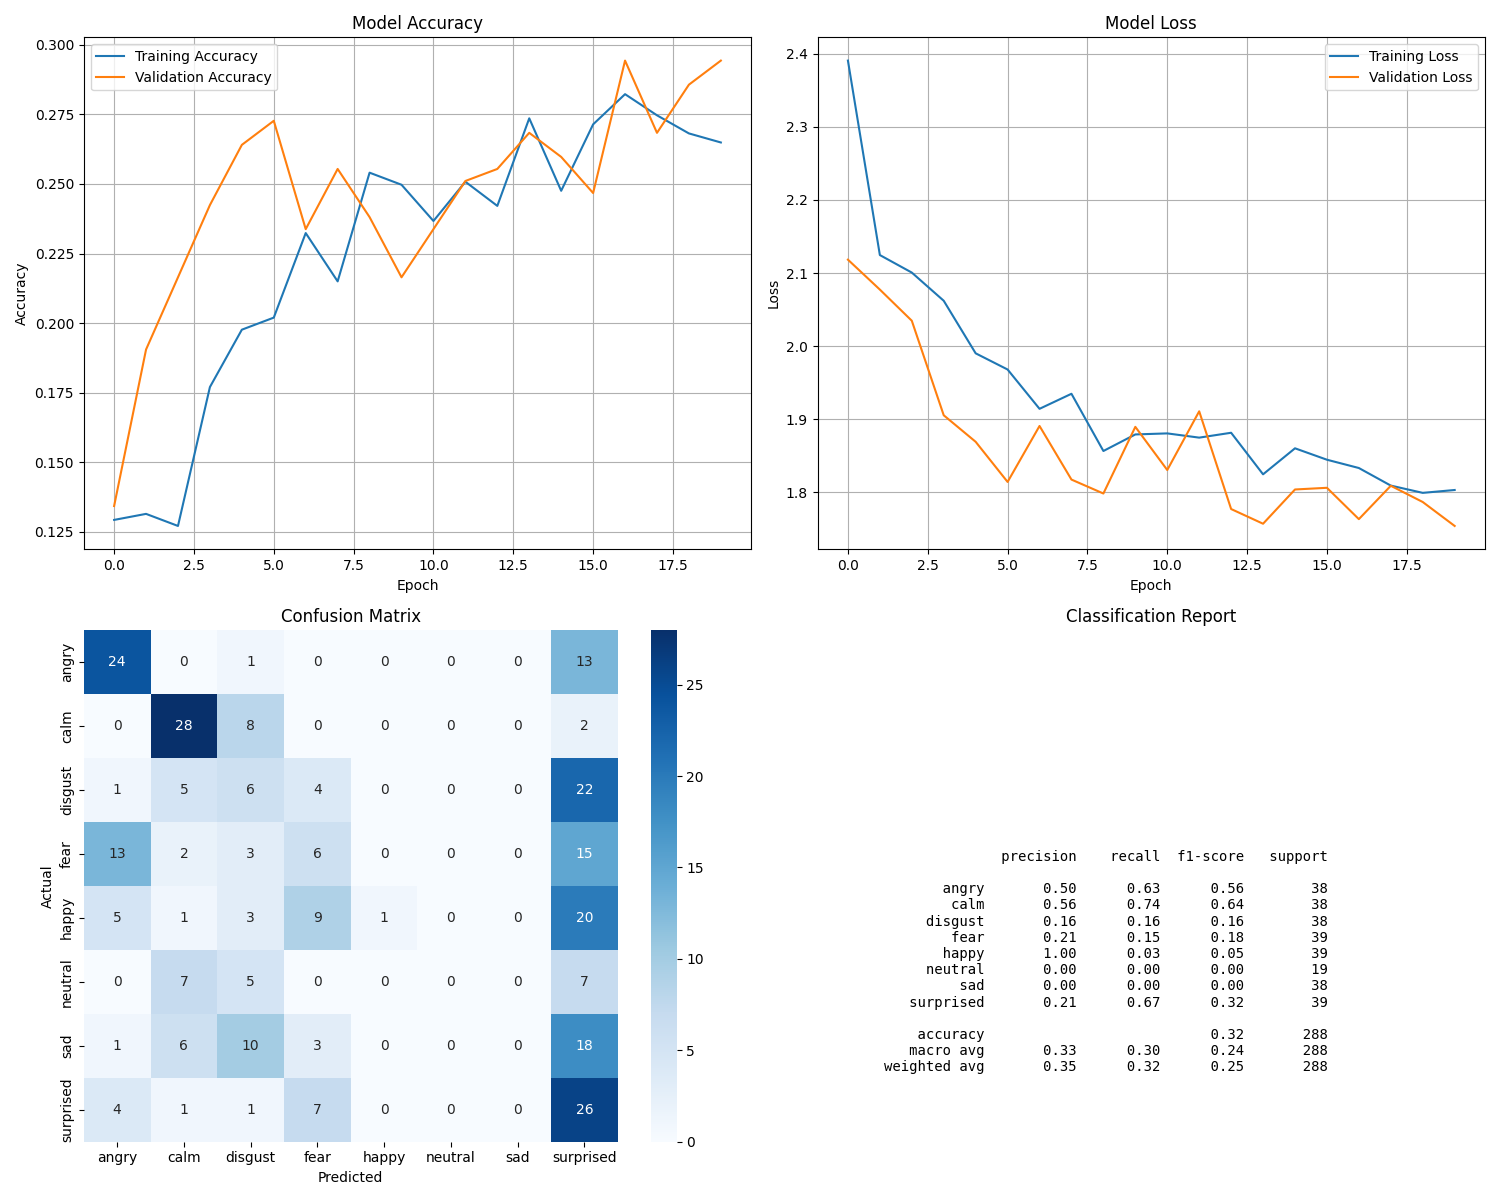
\includegraphics[width=0.3\textwidth]{figures/nuhashmodel1cremad.png}\\[0.3em]
    \caption{Evaluation metrics for the ... model on CREMA-D}
    \label{fig:initial}
\end{figure}


\begin{itemize}
    \item \textbf{Model:}
    \begin{itemize}
        \item Ensemble architecture combining CNN (for spectral features), GRU, and BiLSTM with attention (for sequential features)\cite{electronics10101163}
        \item Inputs: MFCCs, Mel-spectrogram, and Chroma features extracted from audio
        \item (here)Trained and evaluated on the CREMA-D dataset (7 emotions)
    \end{itemize}
    \item \textbf{Results:}
    \begin{itemize}
        \item Moderate accuracy (32\%) on the test set
        \item Confusion matrix shows frequent misclassification among low-arousal emotions (e.g., sad, neutral, disgust)
        \item Training curves indicate stable learning with a minor generalization gap
        \item Model struggles to distinguish subtle differences between similar emotions, especially in challenging classes
    \end{itemize}
\end{itemize}
\end{block}


\begin{block}{Proposed Model and Results}

   \begin{figure}[h!]
        \centering
        \begin{minipage}[b]{0.49\textwidth}
            \centering
            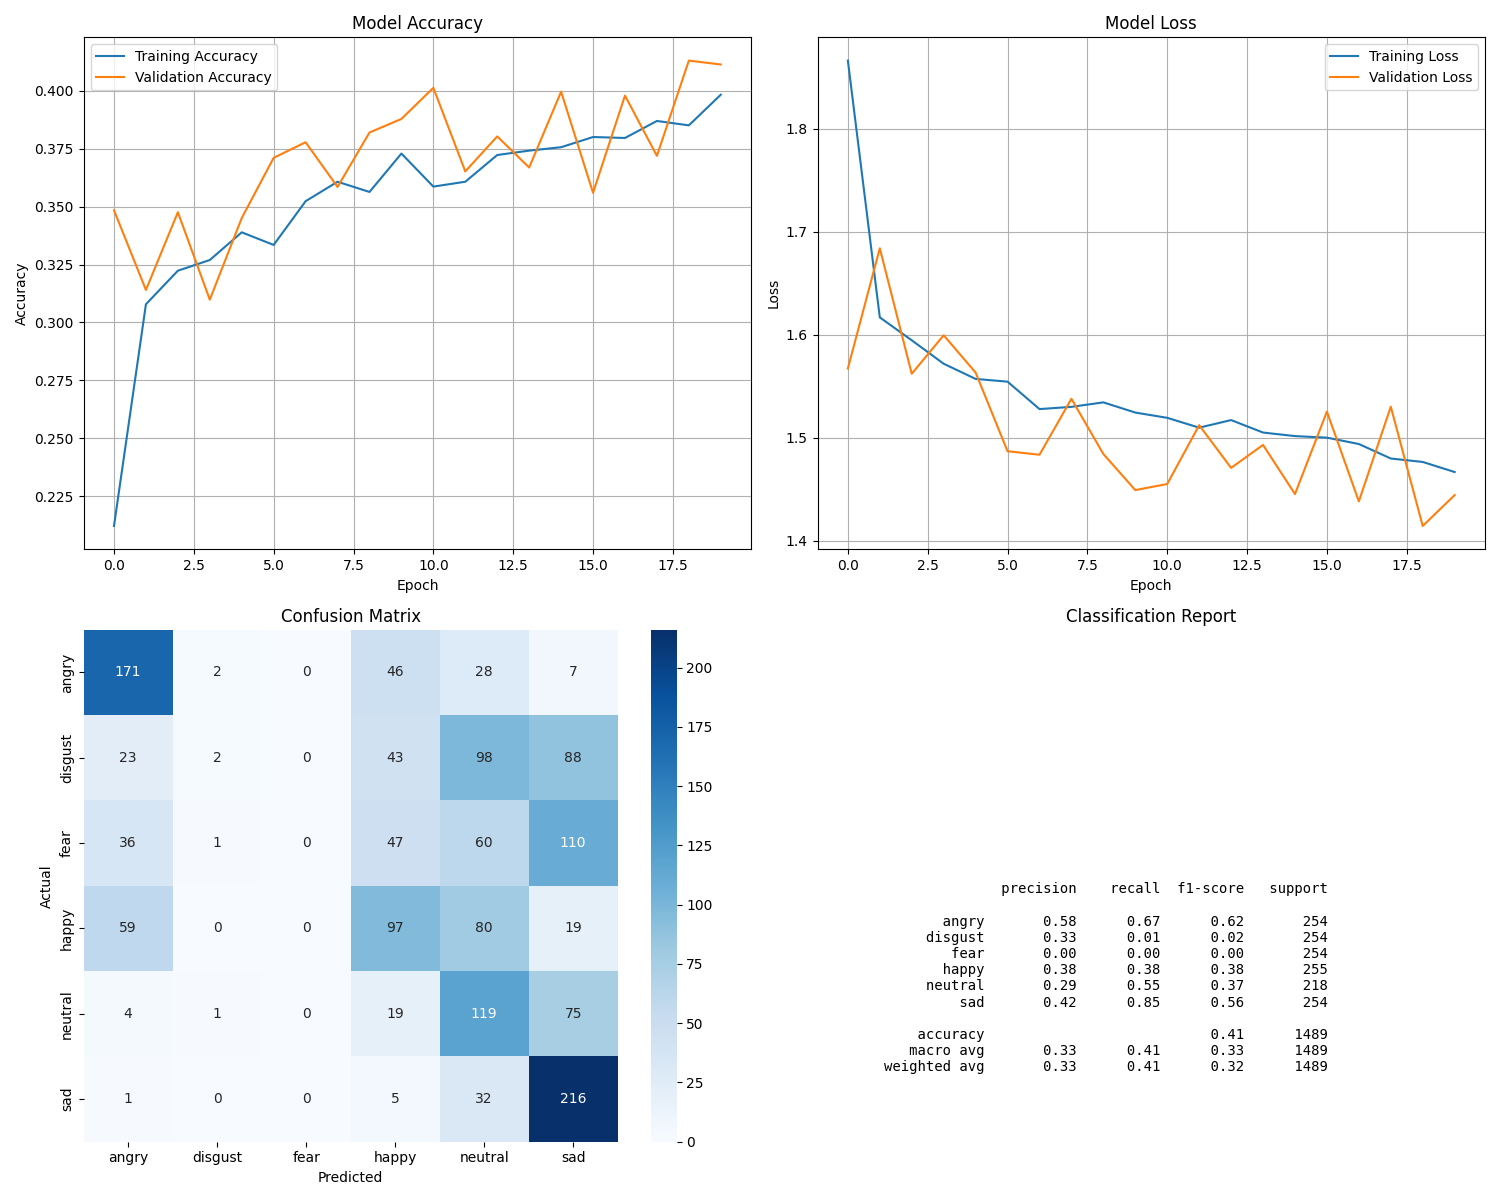
\includegraphics[width=0.5\textwidth]{figures/nuhashmodelfuzzycremadeval.png} % Adjust the height value as needed
            \caption{Evaluation metrics for applying fuzzy c after initial model on CREMA-D}
            \label{fig:fuzzycremaeval}
        \end{minipage}
        \hfill
        \begin{minipage}[b]{0.49\textwidth}
            \centering
            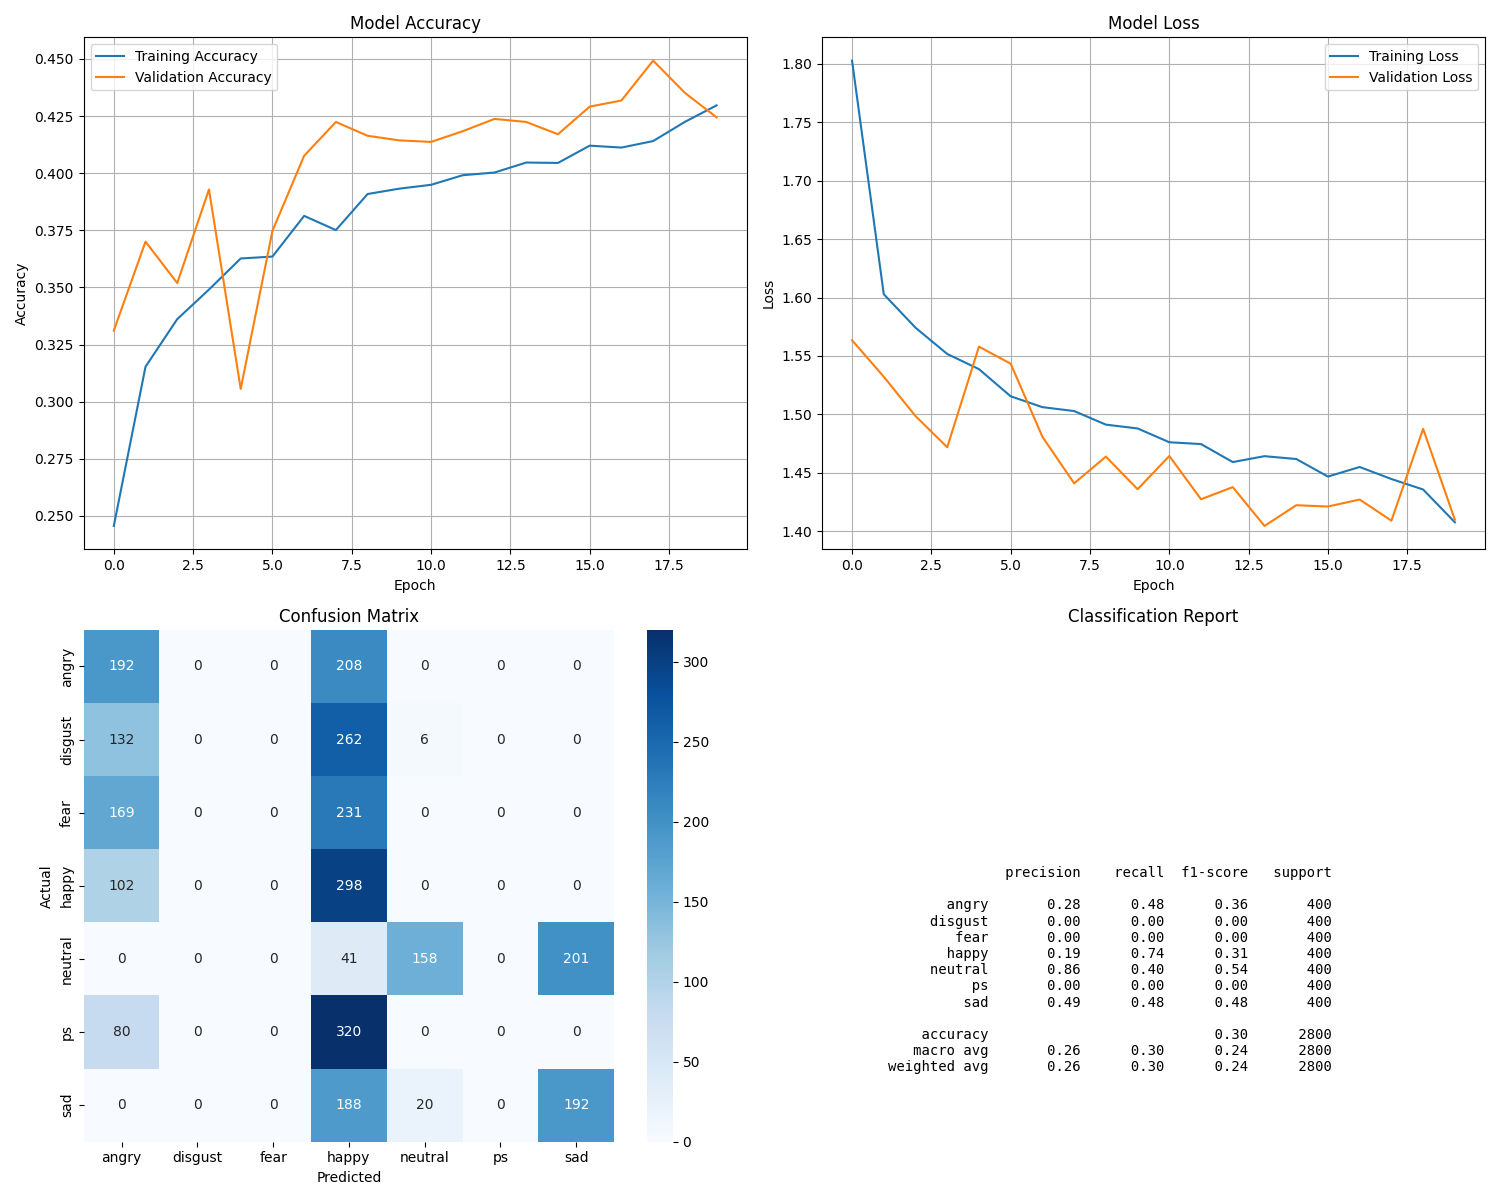
\includegraphics[width=0.5\textwidth]{figures/cremad-tesseval.png} % Adjust the height value as needed
            \caption{Evaluation metrics for applying fuzzy c after initial model on CREMA-D/TESS cross corpus}
            \label{fig:fuzzycrematess}
        \end{minipage}
    \end{figure}

    \begin{figure}[h!]
        \centering
        \begin{minipage}[b]{0.49\textwidth}
            \centering
            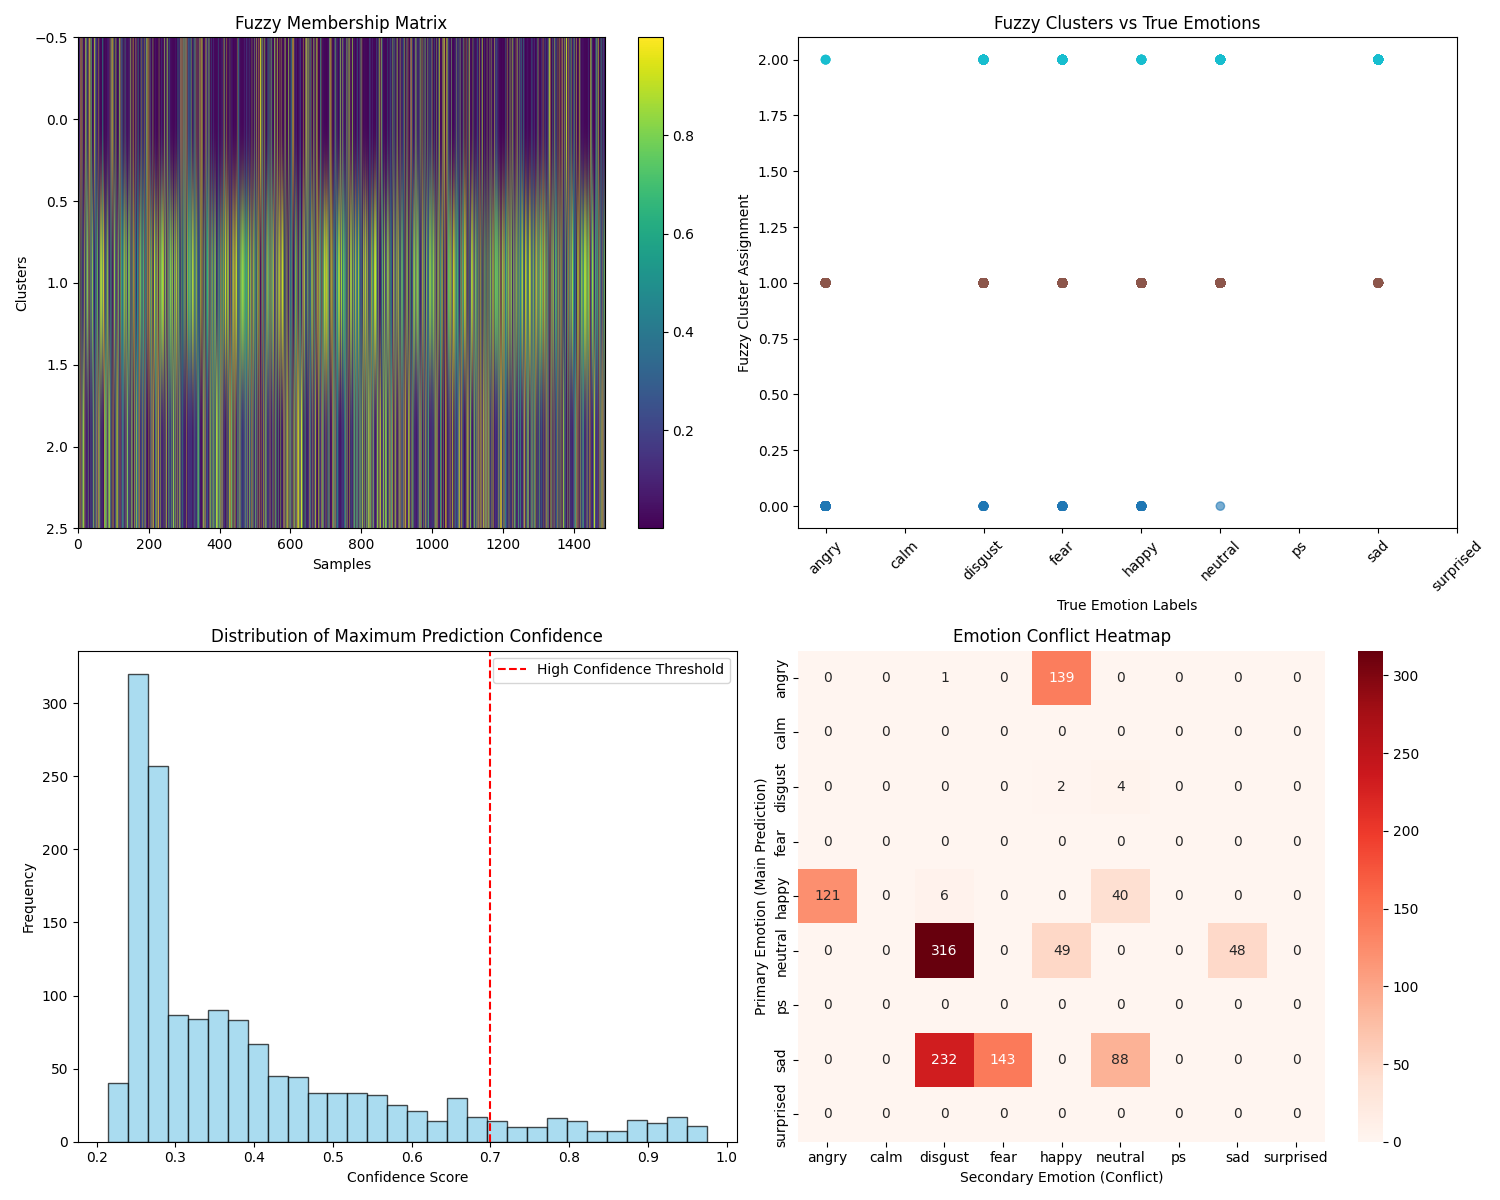
\includegraphics[width=0.5\textwidth]{figures/nuhashmodelfuzzycremad.png} % Adjust the height value as needed
            \caption{Visualization of fuzzy clustering and conflict analysis on model predictions}
            \label{fig:fuzzyviscrema}
        \end{minipage}
        \hfill
        \begin{minipage}[b]{0.49\textwidth}
            \centering
            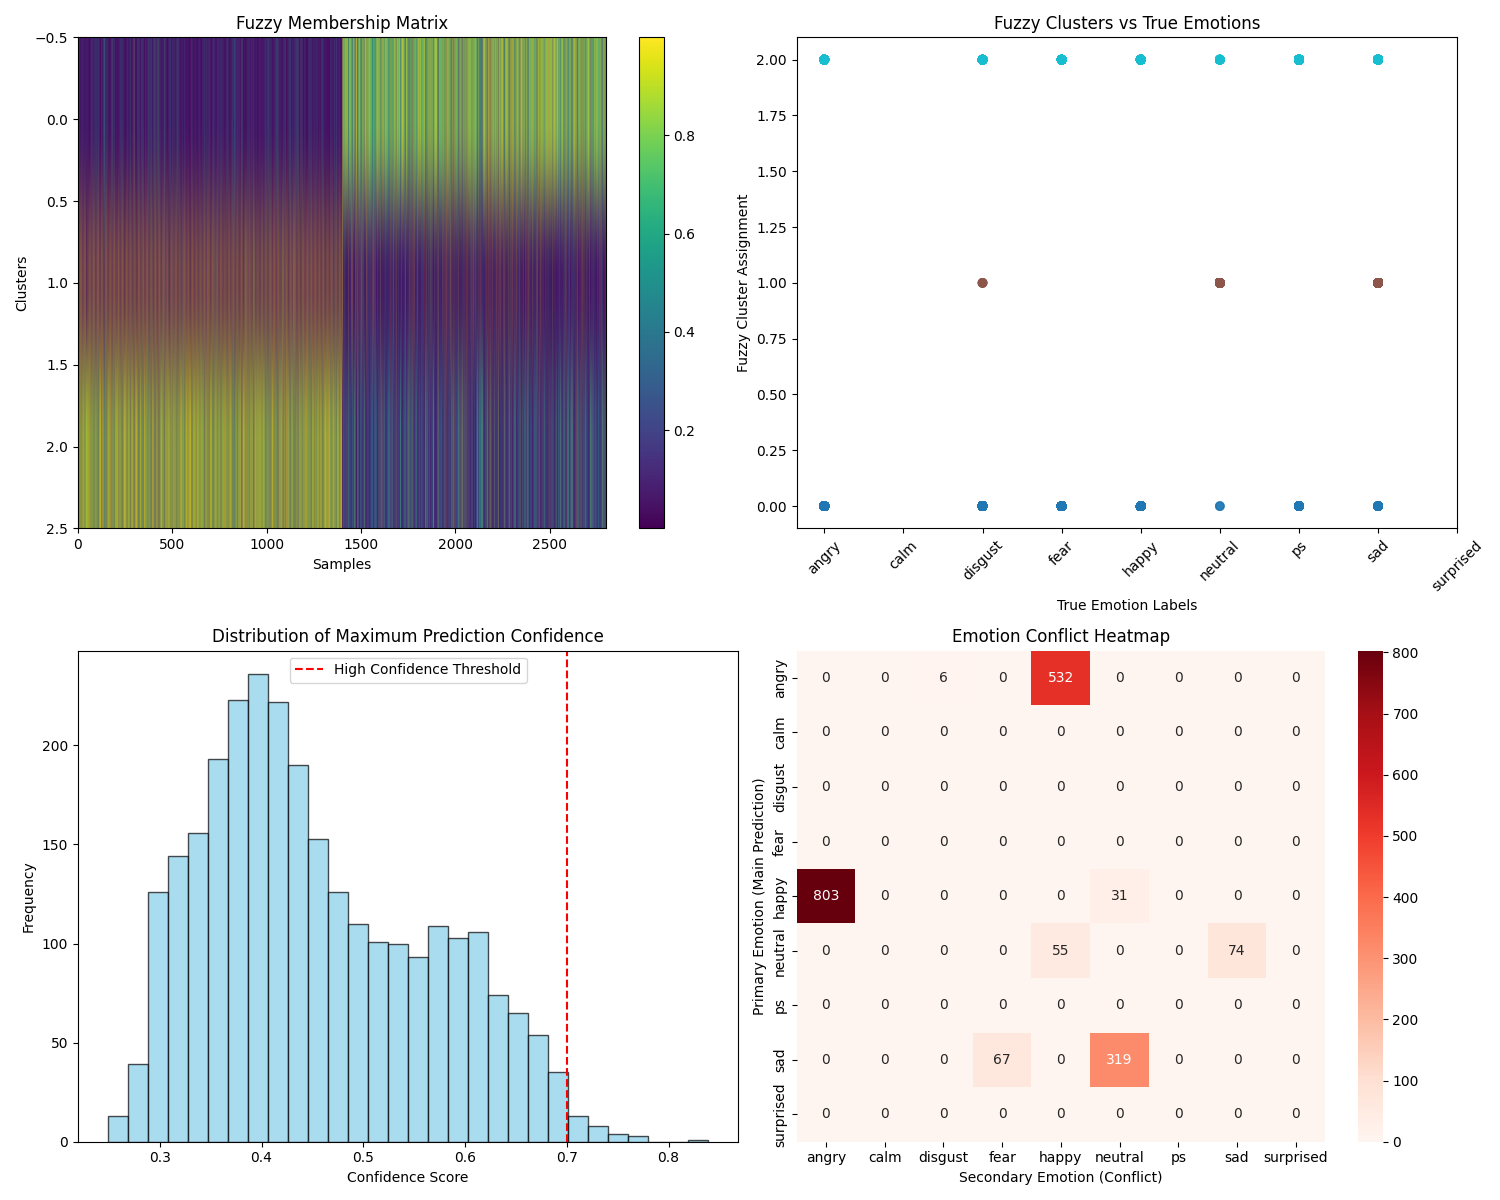
\includegraphics[width=0.5\textwidth]{figures/cremad-tess.png} % Adjust the height value as needed
            \caption{Visualization of fuzzy clustering and conflict analysis on model predictions}
            \label{fig:fuzzyviscrematess}
        \end{minipage}
    \end{figure}

    \vspace{-1cm}
   \begin{itemize}
    \item \textbf{Model:}
    \begin{itemize}
        \item Added Fuzzy C-means clustering to classify emotions better
        \item Inputs: MFCCs, Mel-spectrogram, and Chroma features extracted from audio
        \item (here)Trained and evaluated on the CREMA-D dataset (7 emotions), in addition to cross corpus train-test using CREMA-d and TESS respectively
    \end{itemize}
    \item \textbf{Results:}
    \begin{itemize}
        \item Improved accuracy (41\%) on the test set (CREMA-D), and 30\% on the cross corpus run (trained on CREMA-D, tested on TESS)
        \item Confusion matrix shows significant improvement on the low-arousal emotions 
        \item Training curves indicate more stable learning with a lesser generalization gap
        \item Model distinguishes subtle differences between similar  emotions significantly better
    \end{itemize}
    \end{itemize}




  \end{block}

\end{minipage}
% --- Right Column ---
\begin{minipage}[t]{0.28\textwidth}
\begin{block}{Analysis}

\textbf{Final model -- CREMA-D}
\begin{itemize}    
    \item \textbf{Accuracy:} Moderate (41\%).
    \item \textbf{Confusion Matrix:} Misclassification occurs among fear, disgust, and sadness as a result of overlapping acoustic characteristics.
    \item \textbf{Training Curves:} Learning is stable, despite a minor generalization gap.
\end{itemize}
\textbf{Analysis:} The performance is moderate, due to the dataset's large size and diverse emotional intensity. It still faces difficulties in distinguishing subtle differences between low-arousal emotions (e.g., sadness versus neutral). This further emphasizes the challenges associated with nuanced emotion recognition, even within well-annotated datasets.

\textbf{Final model cross corpus with CREMA-D}
\begin{itemize}
    \item \textbf{Accuracy:} Notable decline (approximately 30\%).
    \item \textbf{Confusion Matrix:} Higher misclassification rates (e.g., distinguishing between happy and neutral).
    \item \textbf{Fuzzy Clustering:} Indicates emotional overlap, particularly within TESS’s older female vocal samples.
\end{itemize}
\textbf{Analysis:} Poor generalization attributed to demographic discrepancies (CREMA-D: varied ages and genders; TESS: exclusively older females). The distinct vocal characteristics of TESS contrast with the more naturalistic recordings found in CREMA-D. This highlights the cross-corpus difficulties faced in practical applications.

\end{block}

\begin{block}{Conclusion}
\begin{itemize}
\item Our hybrid model enhances speech emotion recognition (SER) by identifying overlapping emotions; however, it encounters generalization gaps stemming from biases within the dataset.
\item Future research will focus on attempting to broaden demographic diversity, and enhancing interpretability for practical applications.  
\end{itemize}

\end{block}

\begin{block}{References}

\vspace{-0.2cm}

\nocite{*}
\footnotesize{
\begin{thebibliography}{9}
    \bibitem{electronics10101163}
     E. Lieskovská et al., *A Review on Speech Emotion Recognition Using Deep Learning and Attention Mechanism*, Electronics, vol. 10, no. 10, p. 1163, 2021.\\
    \url{https://www.mdpi.com/2079-9292/10/10/1163}

\end{thebibliography}
}
\end{block}
\end{minipage}

\end{frame}
\end{document}